% !TEX root = Main.tex
\appendix
\appendixpage
\addappheadtotoc
\section{Additional figures}\label{appfigs}
\begin{figure}[h]
	\centering
	\begin{subfigure}[b]{0.3\textwidth}
		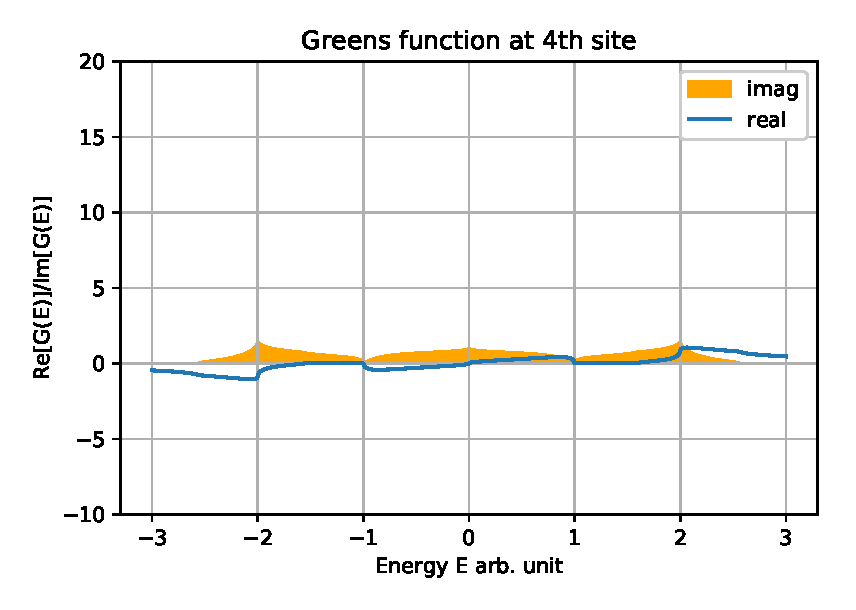
\includegraphics[width=\textwidth]{Figures/BetaimrealTE4.eps}
		\caption{Figure showing a plot of the Green's function at the 4th site}
		\label{4th}
	\end{subfigure}
	~ %add desired spacing between images, e. g. ~, \quad, \qquad, \hfill etc.
	%(or a blank line to force the subfigure onto a new line)
	\begin{subfigure}[b]{0.3\textwidth}
		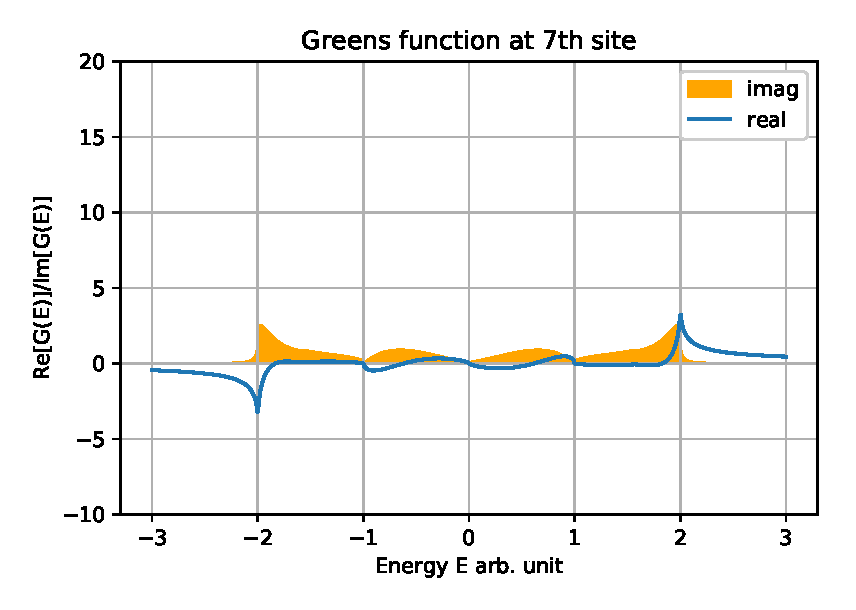
\includegraphics[width=\textwidth]{Figures/BetaimrealTE7.eps}
		\caption{Figure showing a plot of the Green's function at the 7th site}
		\label{7th}
	\end{subfigure}
	\caption{Two plots showing how the Green's function changes as the site is changed. The 4th and 7th sites are corresponding to atoms of those indices (4, 7) in \cref{pointplot}. Note how the LDOS changes (imaginary part) for the different sites.}\label{siteLDOSplot}
\end{figure}
\begin{figure}
	\centering
	\begin{subfigure}[b]{0.3\textwidth}
		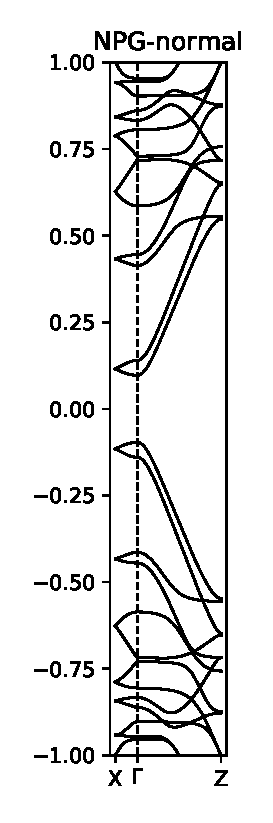
\includegraphics[width=\textwidth]{Figures/FabNPGBS.eps}
		\caption{Plot showing the band structure in the energy range -1 to 1 for NPG with normal bridges between symmetry points \(X\) and \(Z\) with respect to \(\Gamma\)}
		\label{Fabbs}
	\end{subfigure}
	~ %add desired spacing between images, e. g. ~, \quad, \qquad, \hfill etc.
	%(or a blank line to force the subfigure onto a new line)
	\begin{subfigure}[b]{0.3\textwidth}
		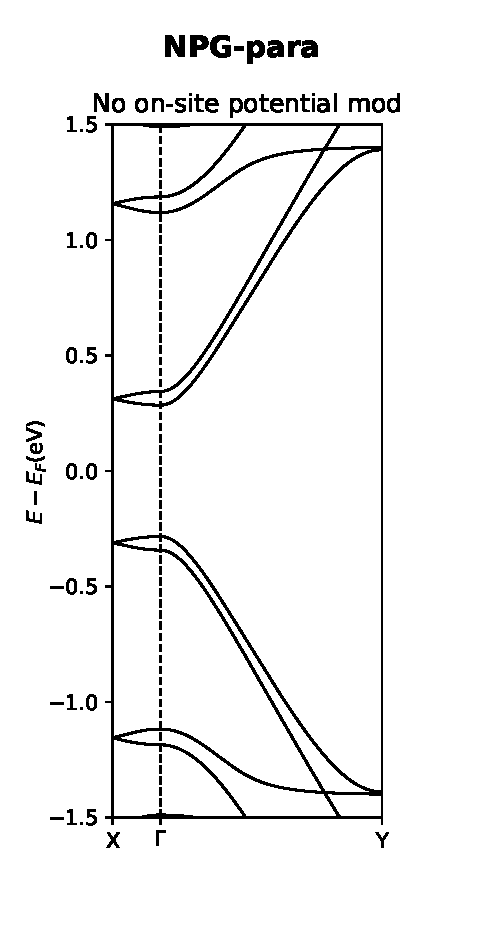
\includegraphics[width=\textwidth]{Figures/paraNPGBS.eps}
		\caption{Plot showing the band structure in the energy range -1 to 1 for NPG with para bridges between symmetry points \(X\) and \(Z\) with respect to \(\Gamma\)}
		\label{parabs}
	\end{subfigure}
	~ %add desired spacing between images, e. g. ~, \quad, \qquad, \hfill etc.
	%(or a blank line to force the subfigure onto a new line)
	\begin{subfigure}[b]{0.3\textwidth}
		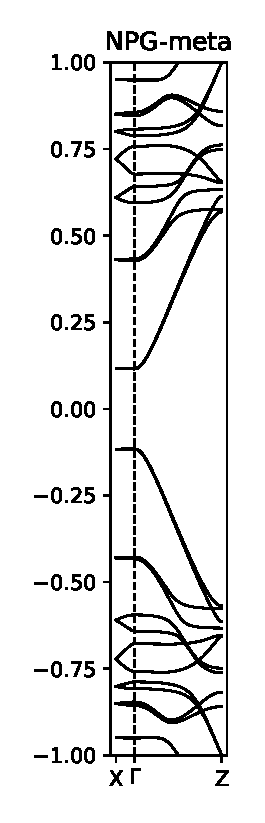
\includegraphics[width=\textwidth]{Figures/metaNPGBS.eps}
		\caption{Plot showing the band structure in the energy range -1 to 1 for NPG with meta bridges between symmetry points \(X\) and \(Z\) with respect to \(\Gamma\)}
		\label{metabs}
	\end{subfigure}
	\caption{Figure showing para, meta and normal NPG band structures}\label{allbands}
\end{figure}
\im{Listings/Functions.py}{41}{47}
\vspace{-1\baselineskip}
\captionof{listing}{Function creating the hopping matrices between two sets of coordinates \label{hopfunc}}\vspace{\baselineskip}

\begin{figure}
	\centering
	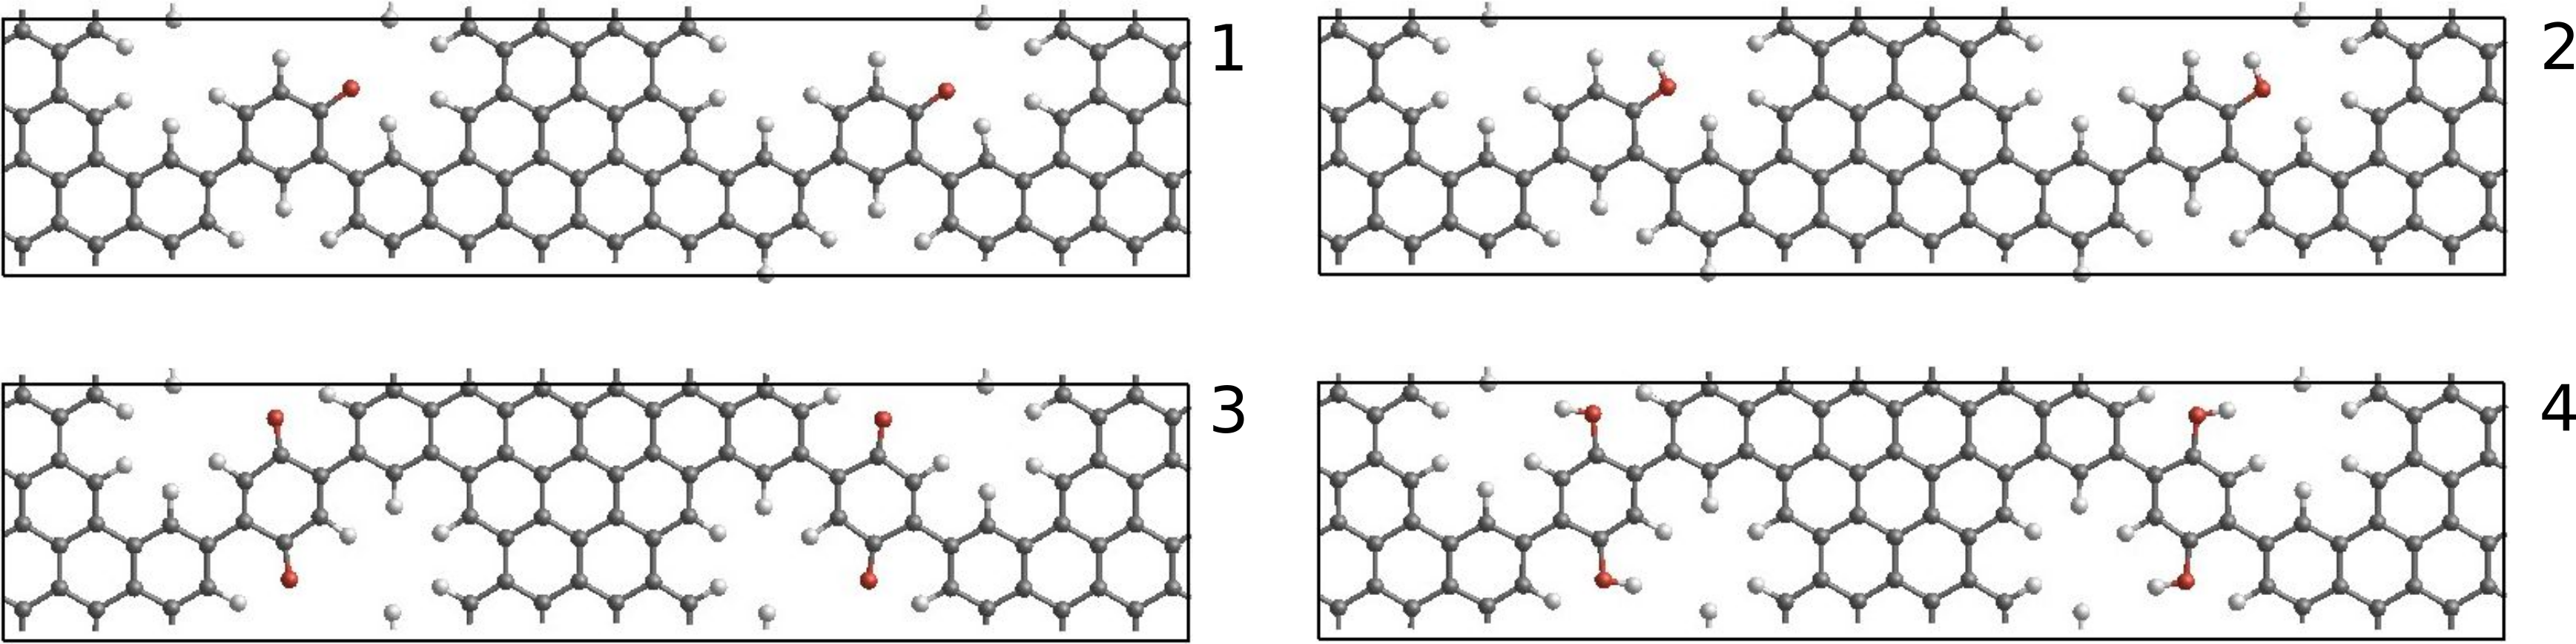
\includegraphics[width=\textwidth]{Figures/Structures.png}
	\caption{Figure showing all the structures stated in \cref{testtable}.}
	\label{Strucow}
\end{figure}

im{Listings/Functions.py}{34}{72}
\vspace{-1\baselineskip}
\captionof{listing}{Code piece showing how the periodic hamiltonian, shifted in the transverse direction i created usind the given unit vector in the y direction.}{\label{periodichamilcode}}\vspace{\baselineskip}

im{Listings/Functions.py}{34}{72}
\vspace{-1\baselineskip}
\captionof{listing}{Code piece showing the line that calculates the transmission}{\label{transmissioncode}}\vspace{\baselineskip}

% \section{Project overview}
% A Gantt chart is provided on the next page. \textbf{Not Updated.}
% \newpage
% \begin{turnpage}
% \setcounter{myWeekNum}{6}
% \ganttset{%
% 	calendar week text={\myWeek{}}%
% }
% \begin{figure}\vspace{-10mm}
% \begin{ganttchart}[
% 		hgrid,
% 		vgrid={*{6}{draw=none}, dotted},
% 		x unit=.15cm,
% 		%	y unit title=.6cm,
% 		%	y unit chart=.6cm,
% 		inline,
% 		milestone inline label node/.append style={left=5mm},
% 		milestone/.append style={xscale=3},
% 		time slot format=isodate,
% 		time slot format/start date=2019-02-04
% 	]{2019-02-04}{2019-05-31}
% 	\gantttitlecalendar{year, month=shortname, week}\\
% 	\ganttgroup{Report writing}{2019-02-25}{2019-05-31}\\
% 	\ganttgroup[inline = false]{Course 33442}{2019-02-04}{2019-03-31}\\
% 	\ganttbar{Ch. 1 \& 2}{2019-02-04}{2019-02-17}\\
% 	\ganttlinkedbar[link bulge=2]{Ch. 3}{2019-02-18}{2019-02-24}\\
% 	\ganttlinkedbar[link bulge=2,bar inline label node/.style={right=15pt}]{Ch. 4 \& 5}{2019-02-25}{2019-03-03}\\
% 	\ganttgroup[inline = false]{Python code}{2019-03-04}{2019-03-31}\\
% 	\ganttbar{Py TB scripts}{2019-02-18}{2019-03-17}\\
% 	\ganttlinkedbar[link bulge=2, bar inline label node/.style={right=45pt}]{Small NPG systems simulations}{2019-03-10}{2019-03-31}\\
% 	\ganttmilestone{Proof of Concept with Python}{2019-03-31}\\
% 	\ganttgroup[inline = false]{Large scale TB}{2019-04-01}{2019-04-28}\\
% 	\ganttbar[bar inline label node/.style={left=10pt}]{SISL \& TBtrans tutorial}{2019-04-01}{2019-04-05}\\
% 	\ganttlinkedbar[link bulge=2, bar inline label node/.style={right=50pt}]{Setup NPG variations}{2019-04-06}{2019-04-28}\\
% 	\ganttgroup[inline = false]{Generate data}{2019-04-28}{2019-05-31}\\
% 	\ganttmilestone{Hand in report}{2019-05-31}
% \end{ganttchart}
% \end{figure}
% \end{turnpage}
% \clearpage
% \global\pdfpageattr\expandafter{\the\pdfpageattr/Rotate 90}
